\documentclass[a4paper,11pt]{article}
\usepackage[a4,bmtuk,themeblue]{tuepdfscreen2008}
\usepackage[english]{babel}
\usepackage{amsmath}      % not required in every poster, only those which use amsmath commands (like \DeclareMathOperator)
\usepackage{mathtime}     % This package is not required, it loads Mathtime fonts for mathematical formulas which I prefer.
\setstatustext{
\includegraphics[height=1.2cm]{IMAGe.png}}       % This text is placed in the upper left corner of the poster and can be left empty
\titlelogo[height=4cm]{veronika_details.png}               % You can use this command to insert one logo.

%\titleright{v.cheplygina@tue.nl  http://www.veronikach.com}
%\titleright{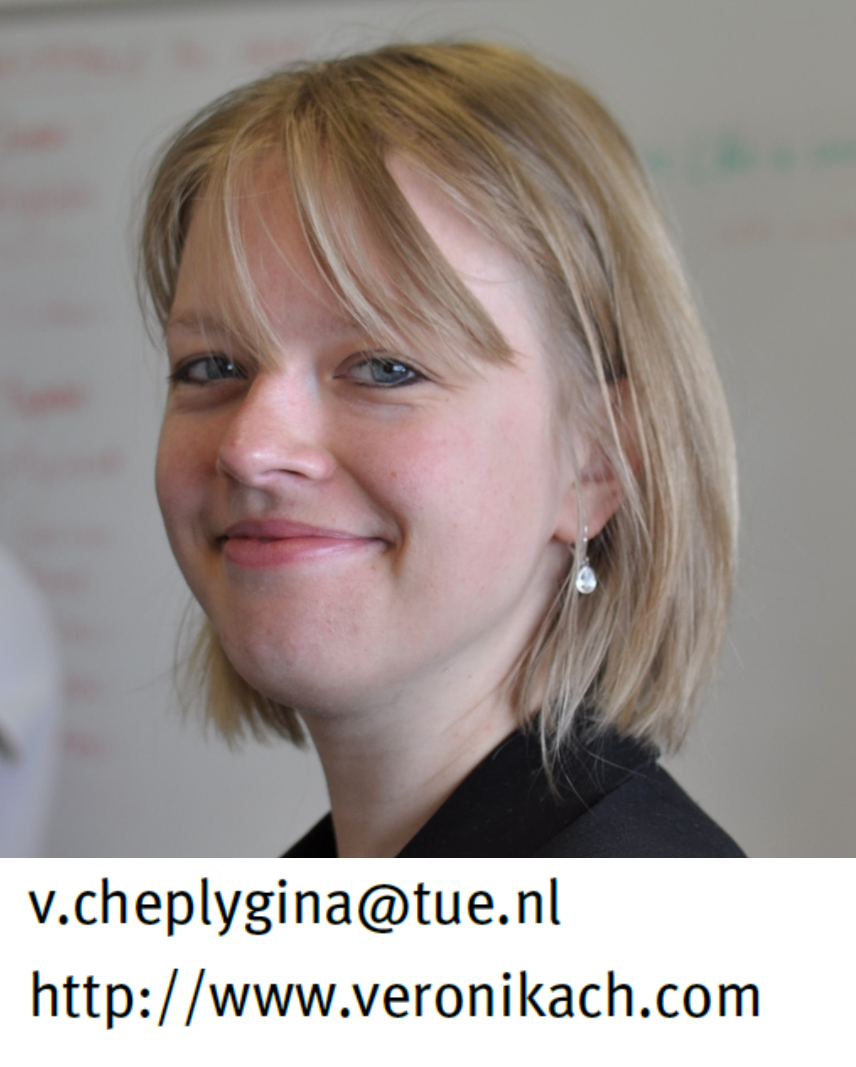
\includegraphics[height=1.2cm]{veronika_details.png}}



\begin{document}
\begin{slidetop}
\slidetitle[Veronika Cheplygina, Adria Perez-Rovira, Wieying Kuo,\\ Harm A. W. M. Tiddens, Marleen de Bruijne]{Crowdsourcing Airway Annotations in Chest CT Images}
\begin{multicols}{2}

\section*{Introduction}

\begin{itemize}
\item Measuring airways important for e.g. cystic fibrosis
\item Measurement is very time-consuming
\item Machine learning methods need annotated data
\item \textbf{Can airway annotations be crowdsourced?}
\end{itemize}

\begin{center}
\includegraphics[width=0.3\columnwidth]{../figures/lungslice.png}
\includegraphics[width=0.3\columnwidth]{../figures/airway_annot.png}
\figcaption{Annotation of an airway in a 2D slice of a CT scan}
\label{fig:airway}
\end{center}


\section*{Crowdsourcing Experiment}

\begin{itemize}
\item 1 CT scan with 76 expert-annotated airways
\item Generate images at expert locations+orientations
\item Amazon MTurk
\item \textbf{Task: annotate airway with 2 ellipses}
\end{itemize}


\begin{center}
\includegraphics[width=0.7\columnwidth]{../figures/flowchart_noicons.png}
\figcaption{Overview of the process}
\label{fig:overview}
\end{center}


\begin{center}
\includegraphics[width=0.7\columnwidth]{../figures/screenshot_testrun2.png}
\figcaption{Instructions to the annotators (notice the scrollbar)}
\label{fig:instr}
\end{center}



\section*{Results}

\begin{itemize}
\item 90 images annotated by 10 workers each
\item Many annotations unusable: 0 or 1 ellipses
\item Usable annotations often good: medium/high correlations with expert
\end{itemize}

\begin{center}
\includegraphics[width=0.9\columnwidth]{../figures/annotation_ellipse.png}
\figcaption{Examples of collected annotations}
\label{fig:airway2}
\end{center}


\begin{center}
\includegraphics[width=0.4\columnwidth]{../figures/scatter_onePair_view1_1.pdf}
\includegraphics[width=0.4\columnwidth]{../figures/scatter_onePair_view1_2.pdf}
\figcaption{Expert vs worker measurements of airway lumen (left) and wall (right)}
\label{fig:individual}
\end{center}

\vspace{0.25cm}

\section*{Discussion}

\begin{itemize}
\item Overall good first experience with crowdsourcing
\item Instructions need to be shorter, simpler
\item Validation on 24 subjects with 20 annotations/image planned
\item Decide locations and orientations without expert?
\item Get more out of unusable annotations?
\item Use annotations to improve machine learning algorithms for airway extraction
\end{itemize}

\footnotesize
Cheplygina, V., Perez-Rovira, A., Kuo, W., Tiddens, H. A., \& de Bruijne, M. (2016). Early Experiences with Crowdsourcing Airway Annotations in Chest CT. Large-Scale Annotation of Biomedical Data and Expert Label Synthesis (MICCAI LABELS) (pp. 209-218).


%\item \texttt{v.cheplygina@tue.nl  \url{http://www.veronikach.com}}

%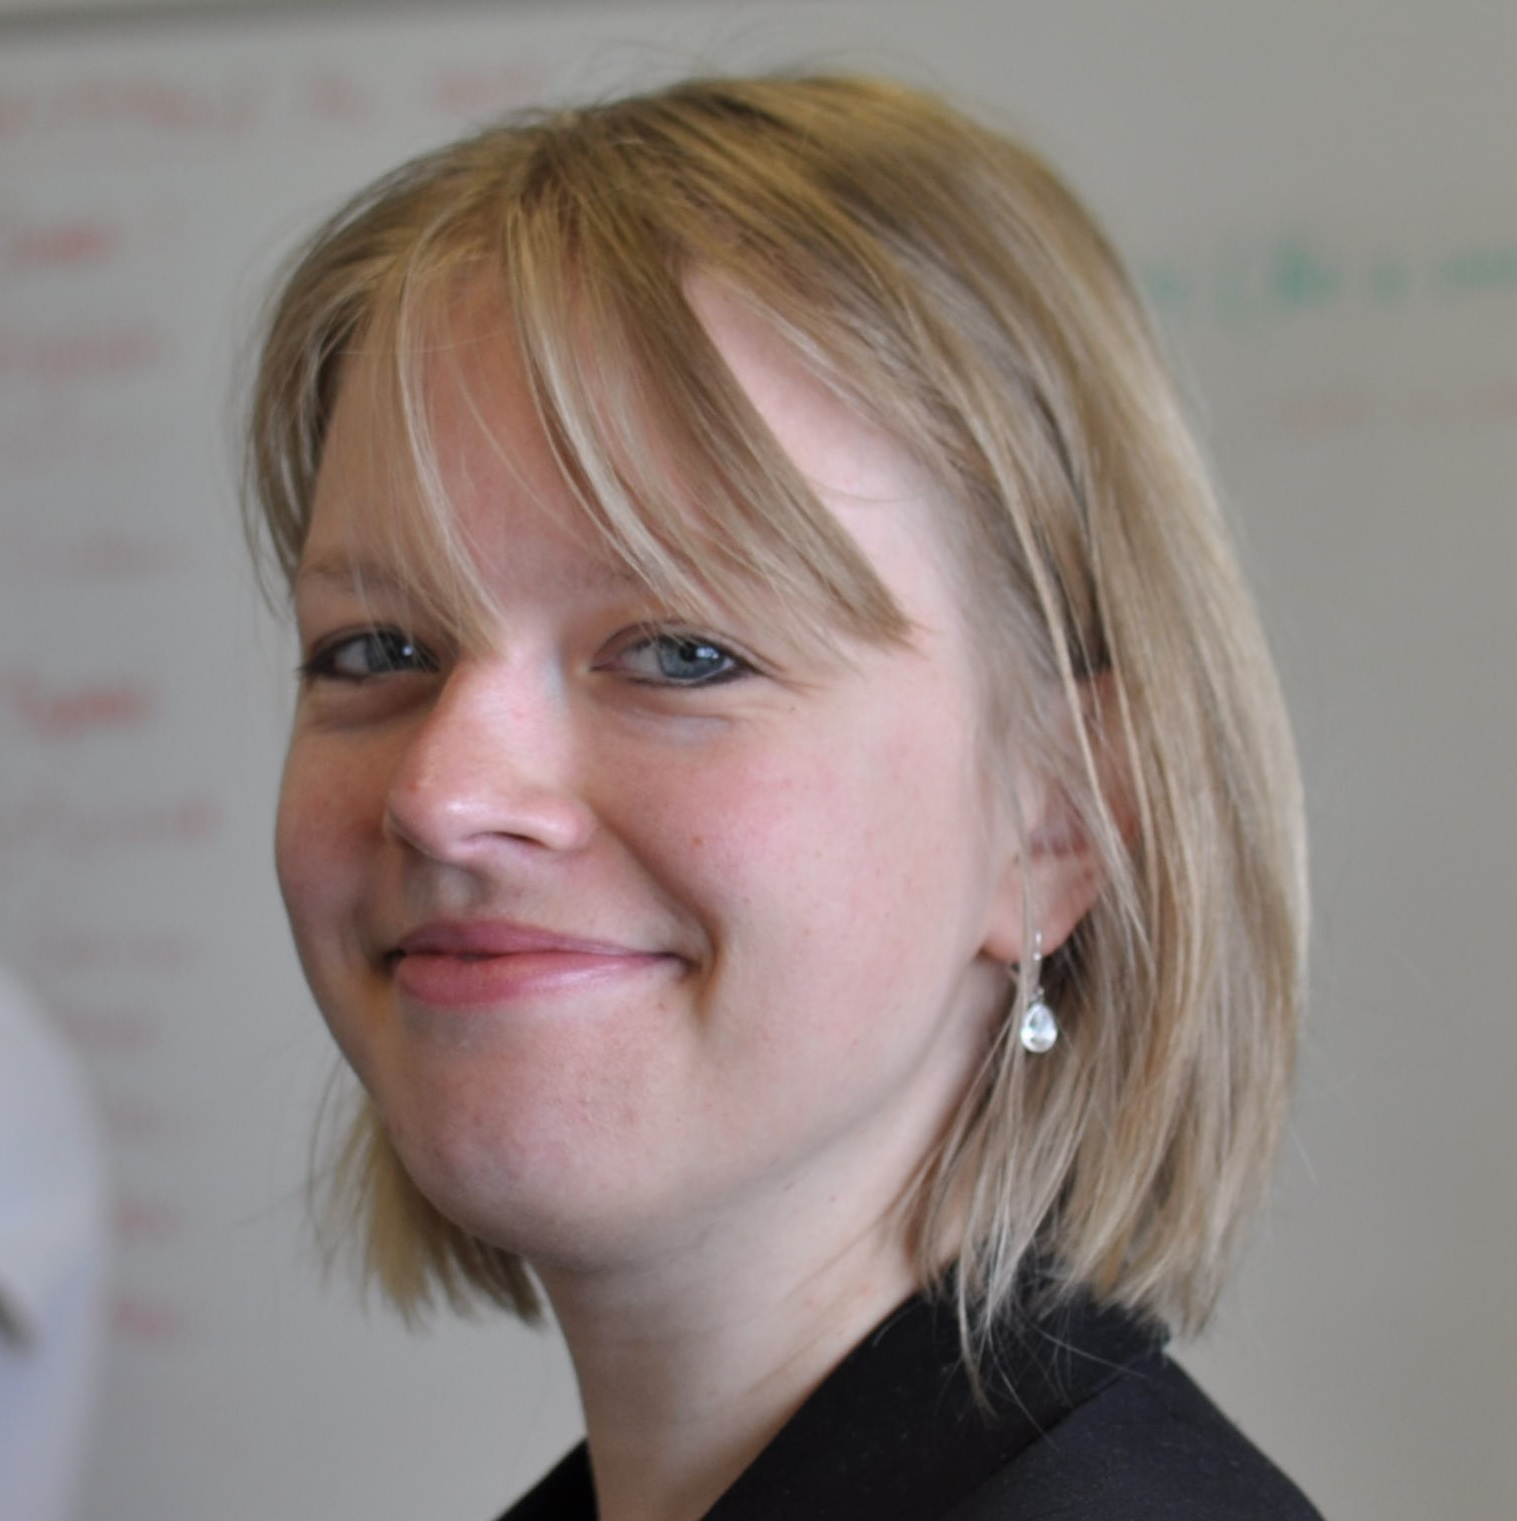
\includegraphics[width=0.2\columnwidth]{../figures/veronika.jpg}
%
\includegraphics[width=0.4\columnwidth]{IMAGe.png}





\end{multicols}
\end{slidetop}

\end{document}

